\documentclass{beamer}
\usepackage{minted}

%Information to be included in the title page:
\title{Sample title}
\author{Siddharth Bhat}
\institute{IIIT Hyderabad}
\date{April 29, 2020}

\begin{document}

\frame{\titlepage}

\begin{frame}[fragile]
\frametitle{The story of a proof: from paper to kernel}
\begin{columns}
\begin{column}{0.5\textwidth}
\begin{figure}[htp]
\centering
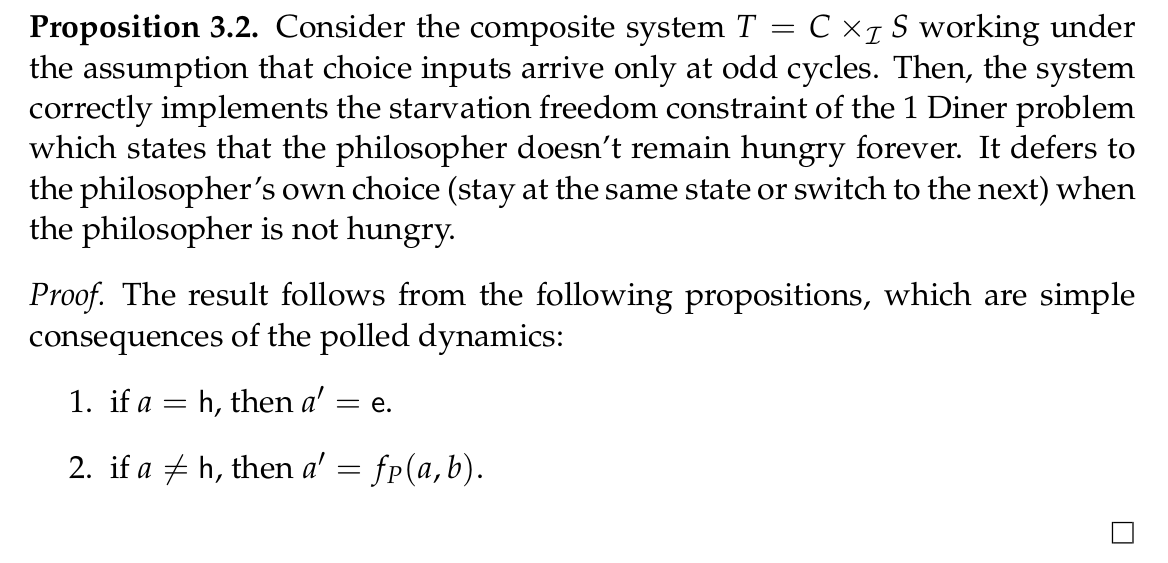
\includegraphics[width=\textwidth]{proposition-starvation-freedom.png}
\end{figure}
\end{column}

\pause

\begin{column}{0.55\textwidth}
{\tiny
\begin{minted}{coq}
Lemma system38_starvation_free:
  forall (n: nat) (ss: nat -> the * cmd)
   (ts: nat -> cmd * maybe choice * the)
   (TRACE_SSSN: ValidTrace system38 ss ts (S(S(S n))))
   (BOTTOM_EVEN: 
      forall (i: nat) (IEVEN: even i = true), 
      snd (fst (ts i)) = nothing choice)
   (NOT_BOTTOM_ODD: 
      forall (i: nat) (IODD: odd i = true),
      snd(fst (ts i)) <> nothing choice)
   (HUNGRY: fst (ss n) = h),
  exists (m: nat),  m > n /\  fst (ss m) = e.
Proof.
    (* 30 lines of proof, 
       200 lines of supporting lemmas ommitted *)
Qed.

Lemma system_38_phil_not_hungry_then_next_philo_choice:
  forall (n: nat) (ss: nat -> the * cmd) (c: choice) 
   (ts: nat -> cmd * maybe choice * the)
   (TRACE_SSSN: ValidTrace system38 ss ts (S(S(S n))))
   (NOTHUNGRY: fst (ss (S n)) <> h)
   (CHOICE: snd (fst (ts (S n))) = just choice c)
   (NEVEN: even n = true)
   (BOTTOM_EVEN: 
     forall (i: nat) (IEVEN: even i = true), 
     snd (fst (ts i)) = nothing choice),
    fst (ss (S(S(S n)))) = trans32fn (fst (ss (S n))) c.
Proof.
    (* 20 lines of proof, 
       200 lines of supporting lemmas ommitted *)
Qed.
  
\end{minted}
}
\end{column}
\end{columns}
\end{frame}


\begin{frame}[fragile]
\frametitle{Statistics}
    \begin{itemize}
            \item  667 lines of coq code.
            \pause
            \item All tables upto section 4 verified by computation.
            \item All theorems upto section 4 formally verified.
    \end{itemize}
\end{frame}

\begin{frame}[fragile]
\frametitle{The definitions: Systems}

{\footnotesize
$$
\text{System} \equiv (X: \textbf{Set}, U: \textbf{Set}, X_0 \subseteq X, \rightarrow \subseteq X \times U \times X).
$$
\pause
    Recall: $X_0 \subseteq X \iff \texttt{member}(X_0): X \rightarrow \texttt{Bool}; ~ \texttt{member}(X_0)(x) \equiv x \underset{?}{\in} X_0$
\pause
\begin{minted}{coq}
(* 2.1: system specifcation *)
Record system (X: Set) (U: Set) := 
    mksystem { isx0: X -> Prop; 
               trans: X -> U -> X -> Prop }.
\end{minted}
}

\end{frame}


\begin{frame}[fragile]
\frametitle{The definitions: Tabuada Connection}

{\tiny
The sets: 
\begin{align*}
    &S \equiv (X: \textbf{Set}, U_X: \textbf{Set}, X_0 \subseteq X, \underset{X}{\rightarrow} \subseteq X \times U_X \times X). \\
    &T \equiv (Y: \textbf{Set}, U_Y: \textbf{Set}, Y_0 \subseteq Y, \underset{Y}{\rightarrow} \subseteq Y \times U_Y \times Y).
\end{align*} }
\pause
{\tiny The interconnect: $$\mathcal I \subseteq (X \times Y) \times (U_X \times U_Y)$$ }
\pause
{\tiny
The composition: 
\begin{align*}
    &S \times_{\mathcal I} T \equiv 
     (Z \equiv X \times Y, U_Z \equiv U_X \times U_Y,  X_0 \times Y_0, \underset{Z, \mathcal{I}}{\rightarrow} \subseteq Z \times U_Z \times Z). \\
    &(x, y) \underset{Z, \mathcal I}{\xrightarrow{u_x,u_y}} (x', y') \iff 
      x \xrightarrow{u_x} x' \land 
      y \xrightarrow{u_y} y' \land (x, y, u_x, u_y) \in \mathcal I.
\end{align*}
}

\pause

{\tiny
\begin{minted}{coq}
(* 2.2: system composition *)
(* tabuada connection new system *)
Definition tabuada {X Y UX UY: Set} 
    (sx: system X UX) (sy: system Y UY) (connect: X*Y->UX*UY->Prop): system (X*Y) (UX*UY) :=
  mksystem (X*Y) (UX*UY) (tabuada_start (isx0 X UX sx) (isx0 Y UY sy))
           (tabuada_trans connect (trans X UX sx) (trans Y UY sy)).
\end{minted}
}


{\tiny
\begin{minted}{coq}
(* initial state for tabuada composition *)
Definition tabuada_start {X Y: Type} (isx0: X -> Prop) (isy0: Y -> Prop) (x: X * Y): Prop :=
  isx0 (fst  x) /\ isy0 (snd x).

(* transition fn for tabuada composition *)
Definition tabuada_trans {X Y: Type} {UX UY: Type}
    (connect: X*Y->UX*UY->Prop) (transx: X -> UX -> X -> Prop) (transy: Y -> UY -> Y -> Prop)
           (s: X*Y) (u: UX*UY) (s': X*Y): Prop :=
  transx (fst s) (fst u) (fst s') /\
  transy (snd s) (snd u) (snd s') /\
  (connect s u).
\end{minted}
}

\end{frame}

\begin{frame}[fragile]
\frametitle{Pain point: Non determinism}
    \begin{itemize}
            \item Coq has computational ability.
            \item Functions are computational; Relations are not.
            \item Lose a lot of proof automation.
    \end{itemize}

\pause

{\footnotesize
\begin{minted}{coq}
Inductive X: Set := X1 | X2 | X3.  Inductive Y: Set := Y1 | Y2 | Y3. 
\end{minted}
\pause
\begin{minted}{coq}
Definition x2y_fn (x: X): Y :=
  match x with | X1 => Y1 | X2 => Y2 | X3 => Y3 end.
(* Works; computational *)
Lemma x1_to_y1_fn: x2y_fn X1 = Y1. Proof. reflexivity. Qed.
\end{minted}
\pause

\begin{minted}{coq}
Definition x2y_rel (x: X) (y: Y): Prop :=
  (x = X1 /\ y = Y1) \/ (x = X2 /\ y = Y2) \/  (x = X3 /\ y = Y3).
Lemma x1_to_y2_rel: x2y_rel X1 Y1.
Proof.
  try reflexivity. (* Does not work! Not computational *)
  unfold x2y_rel. left. auto.
Qed.
\end{minted}
}
\end{frame}

\begin{frame}[fragile]
\frametitle{Pain point: Modularity}
{\tiny
  \begin{minted}[linenos]{coq}
(* Helper:  rewrite ss in terms of ts for the *)
Lemma system38_s_the_to_t_the: 
  forall (n: nat) (ss: nat -> the * cmd) (ts: nat -> cmd * maybe choice * the)
         (TRACE: ValidTrace system38 ss ts (S n)),
    snd (ts n) = fst (ss n).
Proof.
  intros.
  inversion TRACE as [TRACE1 | npred TRACE1 AT1].
  subst.
  inversion AT1 as [AT11 [AT12 AT13]].
  set (s1 := ss 1) in *.
  destruct s1 as [s1_the s1_cmd].
  set (t1 := ts 1) in *.
  destruct t1 as [[t1_cmd t1_mchoice] t1_the].
  simpl in *.
  inversion AT13; simpl in *. (* step where we can see useful info *)
\end{minted}
\pause
\begin{minted}[linenos]{coq}
n : nat
ss : nat -> the * cmd
ts : nat -> cmd * maybe choice * the
TRACE : ValidTrace system38 ss ts (S n)
TRACE1 : ValidTrace system38 ss ts n
AT1 : trans (the * cmd) (cmd * maybe choice * the) system38 (ss n) (ts n) (ss (S n))
AT11 : trans the (cmd * maybe choice) phil37 (fst (ss n)) (fst (ts n)) (fst (ss (S n)))
AT12 : trans cmd the controller34 (snd (ss n)) (snd (ts n)) (snd (ss (S n)))
AT13 : connect38 (ss n) (ts n)
s1_the : the
s1_cmd, t1_cmd : cmd
t1_mchoice : maybe choice
t1_the : the
============================
snd (ts n) = fst (ss n)
\end{minted}
}
\end{frame}

\begin{frame}[fragile]
\frametitle{Lemmas to drive reasoning}

\begin{columns}[T] % align columns
\begin{column}{.48\textwidth}
{\tiny
\begin{minted}{coq}
(* Helper: reason about even/odd *)
Lemma even_n_odd_Sn: forall (n: nat),
    (even n = true) <-> (odd (S n) = true).
(* Helper: reason about even/odd *)
Lemma odd_n_even_Sn: forall (n: nat),
    (odd n = true) <-> (even (S n) = true).
(* Rewrite ts in terms of ss *)
Lemma s_cmd_to_t_cmd: 
  forall (n: nat) (ss: nat -> the * cmd)
    (ts: nat -> cmd * maybe choice * the)
    (TRACE: ValidTrace system38 ss ts (S n)),
    fst (fst (ts n)) = snd(ss n).
(* Rewrite ss in terms of ts *)
Lemma s_the_to_t_the: 
  forall (n: nat) (ss: nat -> the * cmd)
    (ts: nat -> cmd * maybe choice * the)
    (TRACE: ValidTrace system38 ss ts (S n)),
    snd (ts n) = fst (ss n).
(* `h` leads to `!1` command next. *)
Lemma phil_hungry_then_next_controller_bang1:
  forall (n: nat) (ss: nat -> the * cmd)
    (ts: nat -> cmd * maybe choice * the)
    (TRACE_SN: ValidTrace system38 ss ts (S n))
    (HUNGRY: fst (ss n) = h),
    snd (ss (S n)) = cmd_bang1.
\end{minted}
}
\end{column}

\hfill
\begin{column}{.6\textwidth}
{\tiny
\begin{minted}{coq}
(* not `h` in leads to pass next *)
Lemma phil_not_hungry_then_next_controller_pass:
  forall (n: nat) (ss: nat -> the * cmd)
    (ts: nat -> cmd * maybe choice * the)
    (TRACE_SN: ValidTrace system38 ss ts (S n))
    (NOTHUNGRY: fst (ss n) <> h),
    snd (ss (S n)) = cmd_pass.
(* Phil. state in the next-odd-state = cur-state *)
Lemma phil_even_state_next_state:
  forall (n: nat) (ss: nat -> the * cmd)
    (ts: nat -> cmd * maybe choice * the)
    (TRACE_SN: ValidTrace system38 ss ts ((S n)))
    (BOTTOM_EVEN: ...)
    (NEVEN: even n = true),
    fst (ss (S n)) = fst (ss n).
(* Phil. state in the cur-odd-state = prev-state *)
Lemma phil_odd_state_prev_state:
  forall (n: nat) (ss: nat -> the * cmd)
    (ts: nat -> cmd * maybe choice * the)
    (TRACE_SN: ValidTrace system38 ss ts ((S n)))
    (BOTTOM_EVEN: ...)
    (SNODD: odd (S n) = true),
    fst (ss (S n)) = fst (ss n).
(* state after odd cycle has taken transition *)
Lemma odd_state_next_phil_state:
  forall (n: nat) (ss: nat -> the * cmd)
    (ts: nat -> cmd * maybe choice * the)
    (TRACE_SN: ValidTrace system38 ss ts ((S n)))
    (BOTTOM_EVEN: ...)
    (SNODD: odd n = true),
    fst (ss (S n)) = trans37fn  (fst (ss n)) (fst (ts n)). 
\end{minted}
}
\end{column}
\end{columns}
\end{frame}


\begin{frame}[fragile]
\frametitle{Thank you}
    All code available at:

    {\tiny
    \color{blue}{\url{https://github.com/bollu/IIIT-H-code/tree/master/softwarefoundations/project}}
    }

\end{frame}

\end{document}
